\newpage
\section{Implementation}
\label{sec:implementation}

\subsection{Laser Setup}

    \subsubsection{Laser Seeding}
    %============================

The laser setup begins with the master laser.  This laser feeds its light into a slave laser which, if properly tuned, will emit light of the same frequency as its master. That slave then feeds into another slave (\emph{Slave \#2}), which is the light source for this setup.  Particularly, there are a series of mirrors which direct the light from the second slave into the third slave.  Setting up this slave requires a particular algorithm (which must be executed before any work can be done each day). \\

\begin{enumerate}
 \item Lock the master laser and first slave.  This is somewhat involved, and beyond the scope of this document.
 \item Set the current on this slave \#2 to a low value, 32mA is used.
 \item Place a power meter at the output of this slave laser.
 \item Adjust the two mirrors feeding master light into the slave, until the power output from the slave laser is maximised.
 \item Unlock the master laser.  Set it to sweep frequency across a wide enough range that the Rb85 and Rb87 absorption features are visible on the master's diagnostic scope.
 \item Make sure that light from the slave laser is fed back to the diagnostic table (via fibre coupling)\footnote{The diagnostic table includes a scope which shows the spectrum of a rubidium sample, and includes provisions for checking the spectral content of the light.  It is a crucial tool for debugging problems with the laser.}  Check with the power meter that >50\% of the slave light is entering the fibre (there are many reasons why the light might not make it this far.
 \item Set the current into the slave to a high value (110.0mA), and gradually decrease it.  Observe that there is a stable frequency window in which the slave can operate, and that adjusting the current moves this window.  Reduce the current of the slave until the laser is stable across all desired features.  The window should be wide enough to contain both the Rb85 and Rb87 transitions.
 \item The master should either be re-locked, or have its frequency sweep set to a useful range.
 \item The laser can now be used for experiments.
\end{enumerate}

    \subsubsection{Laser Sweeping}
    %=============================

The master laser is nominally operated in a \emph{locked frequency} mode.  There is a lock-box which provides this function, and an AOM-based locking system.  This provides a fast (current based) and slow (piezo based) feedback response, which keeps the laser's frequency as stable as possible. \\

However, if this feedback is disabled, the laser will run in an open-loop \emph{frequency sweeping} mode.  The lock box does not change the current, instead it adjusts the laser's frequency with a triangle wave ramp which operates at 50Hz.  This provides frequency sweep which is very slow compared to the locking servo, but fast enough to give a continuous view of the spectral response of the new feedback system.  For example, by sending this beam through a rubidium gas cell, and placing a detector on the far side, a plot of the absorption spectrum of rubidium as a function of frequency is generated. \\

Note that although the sweep speed is fixed (50Hz), the frequency range of the sweep is set manually by tuning a potentiometer.  Thus, measurements of the sweep rate (MHz/s) need to be done on a per-dataset basis.  No attempt was made to reproduce the exact sweep rate between measurements, although some measurements may have been done without adjusting the settings.  For reference, the sweep rate was set to roughly 120MHz/s. \\

    \subsubsection{Fibre Alignment}
    %==============================

In this section an  example algorithm for aligning fibre couplers is presented.  Much alignment was done in the timespan of this project, so it is worth outlining the procedure that was followed. \\

Each beam has four degrees of freedom.  Thus aligning the beams (in two axes) in two locations is sufficient to have the beams perfectly aligned.  This is required for both fibre couplers and cavities. \\

Fibre couplers:

\begin{enumerate}
 \item Use a laser pen\footnotemark to create a narrow beam coming out of the fibre.  This will be used to determine the alignment of the coupler.
 \item Place a transparent IR card near the fibre coupler such that you can see both the pen laser, and the slave laser beam.
 \item Adjust the last mirror before the coupler until these two beams line up precisely.
 \item Place the transparent IR card past the last mirror.
 \item Adjust the fibre coupler until the two beams line up.
 \item Remove the pen laser and IR card.  Attach the power meter to the fibre coupler.  You should see some power.
 \item Adjust the same four degrees of freedom on the mirror and coupler, maximising the power entering the fibre coupler.  These should be small adjustments.
\end{enumerate}

\footnotetext{A laser pen (the lab has one they call they \emph{spaghetti laser}) is a laser used for aligning optics.  It is small, portable, and includes an adapter which a fibre can be plugged into.  It is designed to feed a visible beam out the fibre so that the alignment of the fibre is completely clear.}

\subsection{Optical Table}

\begin{figure}
  \includegraphics[width=\textwidth]{figures/optical_setup.png}
  \centering\caption{Overview of the optical setup, as it is installed on an ancillary optical table.}
  \label{optical_setup}
\end{figure}

\begin{figure}
  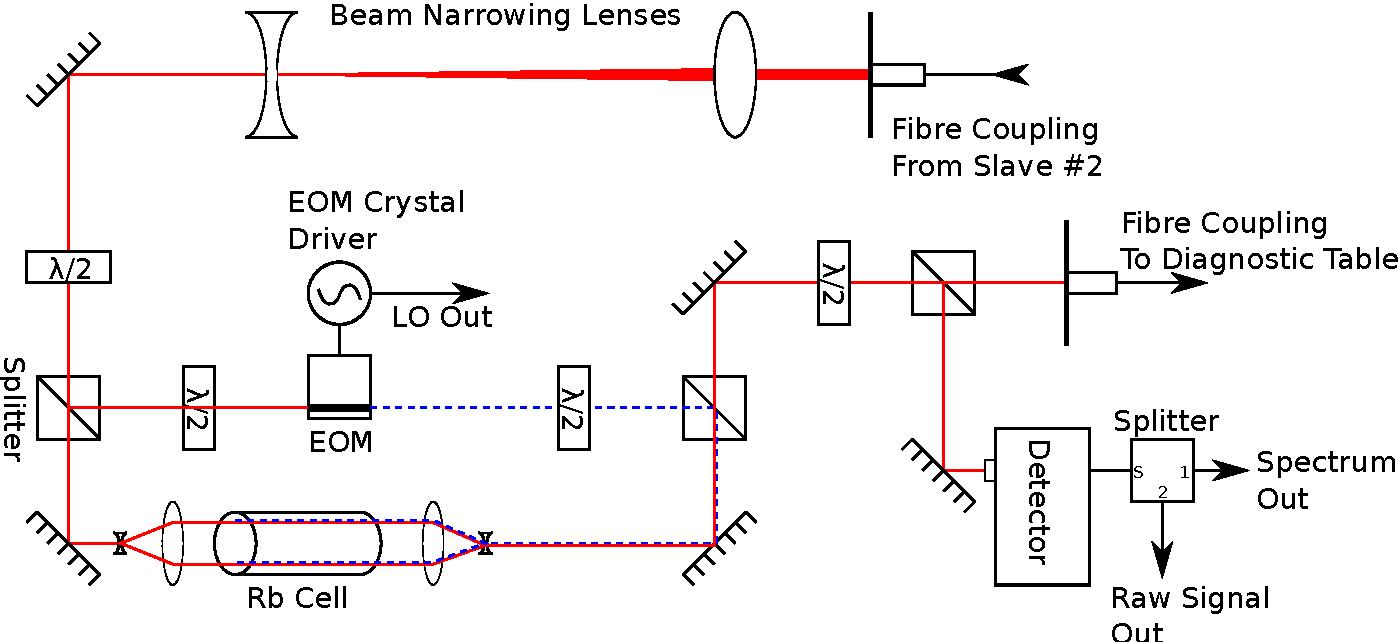
\includegraphics[width=\textwidth]{figures/optics.pdf}
  \centering\caption{A schematic overview of the optical setup.}
  \label{optics}
\end{figure}

An photograph the optical setup is shown in Figure~\ref{optical_setup}.  A schematic view of the same setup is shown in Figure~\ref{optics}.

    \subsubsection{Beam Focusing}
    %============================

The beam that comes out of the fibre coupler spreads too wide over the optical path of the feedback loop.  Thus, a telescope system was installed on the input fiber to reduce the size. A convex lens focusses the beam down, and a concave lens straightens the beam. By moving one of the lenses, the divergence can also be adjusted. This setup was calibrated to have a visibly collimated optical path length of about 2--3 metres. \\

    \subsubsection{Power Control}
    %============================

In several parts of the system, require precise control of beam power.  Specifically, this is needed in three locations: \\

\begin{enumerate}
    \item The power of the pump beam.
    \item The power of the probe beam.
    \item The power distribution between the diagnostic table and the detector.  The detector was visibly saturating in some tests, so this final stage is necessary.  It also makes diagnostics easier if a wide range of power can be arbitrarily redirected to the diagnostic table.
\end{enumerate}

In each of these locations, there is a half-wave plate followed by a pol cube.  The half wave plate rotates the polarization of linear polarized light.  The pol cube allows horizontally polarized light to pass straight through, while reflecting vertically polarized light\footnote{The pol cube does not work with 100\% efficiency—some horizontally polarized light will reflect and some vertically polarized light will pass straight through. This is commonly referred to as the `extinction ratio' and it puts a lower limit on the power levels in a given path}. \\

    \subsubsection{EOM and Crystal Driver}
    %===================================

\begin{figure}
  \includegraphics[width=.5\textwidth]{figures/eom_driver.jpg}
  \centering\caption{The EOM Crystal Driver circuit used.  The attenuation and phase adjustment potentiometers are visible.  Also visible, the output port (to EOM) and the ref output port (to LO).}
  \label{eom_driver}
\end{figure}

An EOM crystal driver was borrowed from the Phys 408 Optics lab.  It is shown in Figure~\ref{eom_driver}.  The availability of a working device greatly reduced the cost overhead of this project.  The driver generates a sinusoidal signal at approximately 20MHz, and is tuned to drive the high capacitance of the EOM crystal at a high voltage.  It also feeds out a reference to its internal oscillator.  This signal provides the local oscillator input for demodulation. \\

The EOM driver also includes a phase shift potentiometer to account for phase shifts that may occur in electrical lines or the optical path.  However, the shift provided by this potentiometer is woefully inadequate, with an approximate range of $\lambda/6$ (at least $\lambda/2$ would be ideal).  A phase delay was manually introduced using BNC cables of various lengths.  Of the cables tried, a 1.5m cable provided the best signal (but this method is clearly suboptimal).  The maximum phase shift of the driver is shown in Figure~\ref{fig:eom_phase}. \\

The light passing into the EOM must be horizontally polarized, thus a half-wave plate is used to re-polarize the light before it enters the EOM. \\

\begin{figure}
  \begin{tabular}{cc}
    \includegraphics[width=0.47\textwidth]{figures/{eom_driver_onboard_1}.jpg} &
    \includegraphics[width=0.47\textwidth]{figures/{eom_driver_onboard_2}.jpg} \\
  \end{tabular}
  \caption{The maximum phase shift of the EOM driver reference output, with no load attached.  Red signal corresponds to the driver (1MΩ), blue signal corresponds to LO out.  The impedance of the load affects the shape of both waveforms.}
  \label{fig:eom_phase}
\end{figure}

    \subsubsection{Pump Probe Modulation Transfer}
    %=============================================

The an EOM-modulated beam is fed into the sample from one direction (the \emph{pump} beam).  A single frequency beam (from the slave laser) passes through the gas in the opposite direction (the \emph{probe} beam).  Due to nonlinear interactions in the gas, the probe beam becomes modulated at the driving frequency of the pump beam.  That is, the pump beam modulates the gas, which in turn, modulates the probe beam. \\

The physics of the interaction between the two beams and the gas are described further in the \textbf{Section \ref{sec:theory}}. \\

Note that the cell has been installed at a slight angle, to minimize reflections off the surface of the cell. \\

    \subsubsection{Rb Cell Beam Expander}
    %====================================

The Rb gas cell has been surrounded in telescoping lenses to expand both the probe and pump beam.  This improves the signal-to-noise ratio by passing the beam through a larger fraction of the gas in the cell.  The telescopes increase the diameter of both beams by a factor of 3. \\

    \subsubsection{Heated Rb Cell}
    %=============================

Heating the rubidium cell can improve the signal to noise of this system.  At room temperature, a fraction of the rubidium in the cell exists as a solid on the surface of the cell.  By heating the cell, more rubidium will vapourize, increasing the density of the gas.  This causes the laser to pass through more gas, which strengthens the signal. \\

However, this effect cannot be used to arbitrary temperatures.  Increasing the temperature increase the vapour pressure, but it also increases the speed of the gas molecules, which causes the Doppler broadening to become worse, until the response ultimately becomes flat.  This effect is known as pressure broadening, and puts an upper limit on the possible performance improvements. \\

Heating was done with a pre-built heating coil and a measured with a K-type thermocouple.  For each temperature measurement, the heater was activated, and it's current load was manually adjusted the current output until the temperature reading on the thermocouple had remained stable for five minutes.  At the point of sampling, the heater was shut off (to eliminate any magnetic fields created by the current), and a measurement of the error signal was taken. \\

    \subsubsection{Cavity Wave Detector}
    %===================================

\begin{figure}
  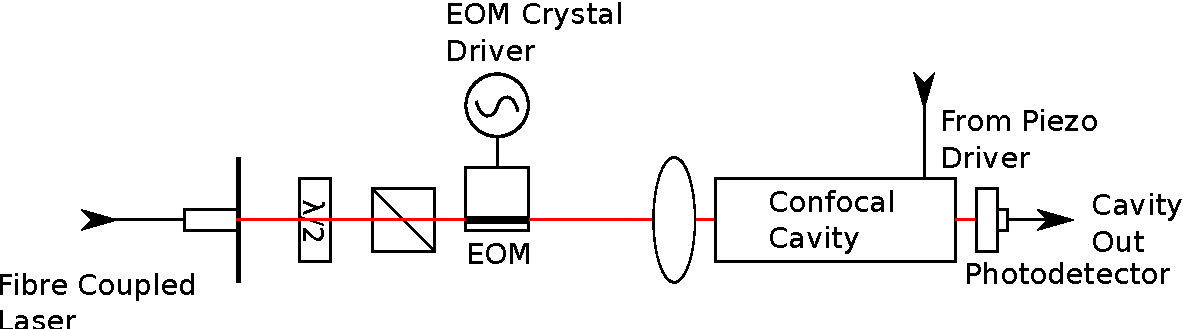
\includegraphics[width=\textwidth]{figures/cavity.pdf}
  \caption{Confocal cavity test setup.  The EOM is passed through a half wave plate, which allows us to adjust its polarization, and then through a pol cube which removes any vertically polarized light, leaving only horizontally polarized light.  The piezo element is fed by a function generator, and the piezo driving force, which corresponds to frequency, is plotted against the response of the photodetector.}
  \label{cavity}
\end{figure}

A confocal cavity was used to measure the effect the EOM has on the beam, to ensure that sidebands are in fact being created.  The setup of this cavity is shown in Figure~\ref{cavity}  The cavity resonates more highly with laser light that fits in an integer number of wavelengths within the cavity.  Having a photodiode on the end allows for measurement of the resonance amplitude.  The backside of the cavity can be moved by adjusting the voltage applied to a piezo system.  By feeding a triangular wave in (from a function generator), the (rough) frequency spectrum of the beam is observed. \\


\begin{figure}
  \centering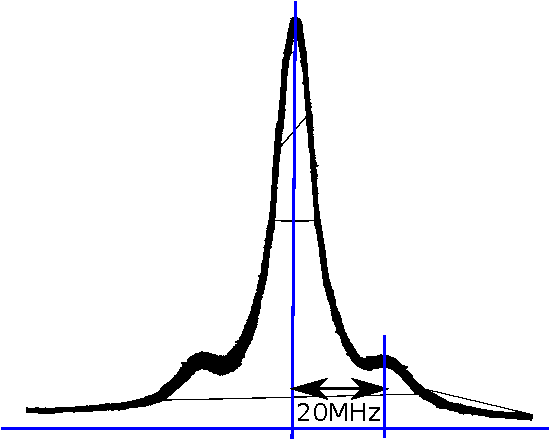
\includegraphics[width=0.5\textwidth]{figures/eom_wave.pdf}
  \caption{EOM Spectrum as viewed from the detector of a confocal cavity.  Sidebands appear on the light wave at ±20MHz from the carrier (which was calibrated from the free spectral range of the cavity). The measured sideband amplitudes were $14\pm1$\% of the carrier, which is approximately a 1:7:1 split of total power.}
  \label{fig:eom_wave}
\end{figure}

Figure~\ref{fig:eom_wave} shows that the EOM driver is functioning correctly. \\

    \subsubsection{Modulation Transfer Reference}
    %============================================

Since the frequency was sweept during the main tests, the low-frequency (near DC) part of the signal was isolated to give an indication of the actual modulation transfer spectrum.  This provided a continuous reference of which part of the spectrum was being sampled at all times. Additionally, this indicated how well the modulation transfer was working. \\

The raw signal itself, which we send off to the signal conditioning box, which converts it into a usable error signal. \\

\subsection{Signal Conditioning}
\label{sec:signalcond}

\begin{figure}
  \centering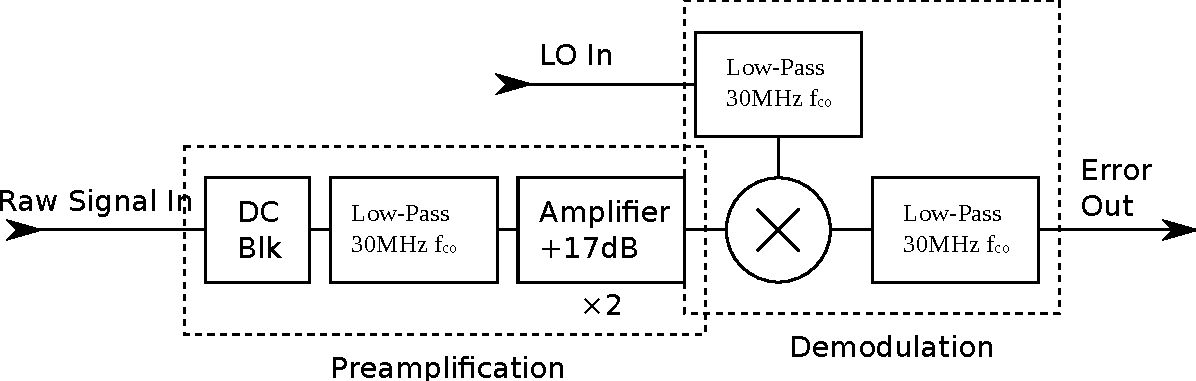
\includegraphics[width=\textwidth]{figures/rf_design.pdf}
  \caption{An overview of the signal conditioning stages.}
  \label{rf_design}
\end{figure}

An overview of the signal conditioning stages is shown in Figure~\ref{rf_design}. \\

    \subsubsection{Preamplification}
    %===============================

The 20MHz signal created at the detector is first filtered.  The DC component and everything above 30MHz are cut out, leaving ideally just the desired 20MHz signal.  That signal gets passed through two 17dB minicircuits RF amplifiers, which increase the power level of the signal enough to make it usable.  Each amplifier degrades the signal-to-noise by 6dB, so excessive chaining amplifiers should be avoided if possible. \\

    \subsubsection{Demodulation}
    %===========================

The preamplified signal is passed into a frequency mixer.  That signal is mixed with the 20MHz local oscillator (the EOM driver).  This gives us a desired signal at DC.  The mixed signal is then filtered at 10MHz, which eliminates any unwanted high frequency components.  The selection of frequency is important at this stage.  The higher a the cutoff frequency, the faster the system can respond to changes in the laser's frequency. However, setting a high frequency incurs a noise penalty.  The noise spread is linear, thus a doubling of frequency range decreases the SNR by 3dB. \\

A 10MHz cutoff frequency was chosen, primarily to eliminate known nonlinear artifacts of the mixer present at 20MHz; these filters reduce a signal at $2f_{co}$ by 40dB\cite{zfl_1000}.  Reducing this cutoff would further reduce the output noise. \\

\subsection{Infrastructure}
    \subsubsection{EOM Power Supply}
    %===============================

The homebuilt EOM driver CCA came with its own AC to DC converter.  However, supply noise proved to be a problem, so a custom power supply was developed for this board.  The power supply takes filtered DC lab power, and linearly downregulates to the needed input power. \\

    \subsubsection{Signal Conditioner Case and Power Distribution}
    %=============================================================

A custom case was built to contain the signal conditioning components.  It also includes a linear regulator which is capable of powering up to 4 of the minicircuits amplifiers.

